%  LaTeX support: latex@mdpi.com
%  In case you need support, please attach all files that are necessary for compiling as well as the log file, and specify the details of your LaTeX setup (which operating system and LaTeX version / tools you are using).

%=================================================================
\documentclass[smartcities,article,submit,moreauthors,pdftex]{mdpi}

% If you would like to post an early version of this manuscript as a preprint, you may use preprint as the journal and change 'submit' to 'accept'. The document class line would be, e.g., \documentclass[preprints,article,accept,moreauthors,pdftex]{mdpi}. This is especially recommended for submission to arXiv, where line numbers should be removed before posting. For preprints.org, the editorial staff will make this change immediately prior to posting.

%% Some pieces required from the pandoc template
\providecommand{\tightlist}{%
  \setlength{\itemsep}{0pt}\setlength{\parskip}{4pt}}
\setlist[itemize]{leftmargin=*,labelsep=5.8mm}
\setlist[enumerate]{leftmargin=*,labelsep=4.9mm}

\usepackage{longtable}

% see https://stackoverflow.com/a/47122900
\usepackage{color}
\usepackage{fancyvrb}
\newcommand{\VerbBar}{|}
\newcommand{\VERB}{\Verb[commandchars=\\\{\}]}
\DefineVerbatimEnvironment{Highlighting}{Verbatim}{commandchars=\\\{\}}
% Add ',fontsize=\small' for more characters per line
\usepackage{framed}
\definecolor{shadecolor}{RGB}{248,248,248}
\newenvironment{Shaded}{\begin{snugshade}}{\end{snugshade}}
\newcommand{\AlertTok}[1]{\textcolor[rgb]{0.94,0.16,0.16}{#1}}
\newcommand{\AnnotationTok}[1]{\textcolor[rgb]{0.56,0.35,0.01}{\textbf{\textit{#1}}}}
\newcommand{\AttributeTok}[1]{\textcolor[rgb]{0.77,0.63,0.00}{#1}}
\newcommand{\BaseNTok}[1]{\textcolor[rgb]{0.00,0.00,0.81}{#1}}
\newcommand{\BuiltInTok}[1]{#1}
\newcommand{\CharTok}[1]{\textcolor[rgb]{0.31,0.60,0.02}{#1}}
\newcommand{\CommentTok}[1]{\textcolor[rgb]{0.56,0.35,0.01}{\textit{#1}}}
\newcommand{\CommentVarTok}[1]{\textcolor[rgb]{0.56,0.35,0.01}{\textbf{\textit{#1}}}}
\newcommand{\ConstantTok}[1]{\textcolor[rgb]{0.00,0.00,0.00}{#1}}
\newcommand{\ControlFlowTok}[1]{\textcolor[rgb]{0.13,0.29,0.53}{\textbf{#1}}}
\newcommand{\DataTypeTok}[1]{\textcolor[rgb]{0.13,0.29,0.53}{#1}}
\newcommand{\DecValTok}[1]{\textcolor[rgb]{0.00,0.00,0.81}{#1}}
\newcommand{\DocumentationTok}[1]{\textcolor[rgb]{0.56,0.35,0.01}{\textbf{\textit{#1}}}}
\newcommand{\ErrorTok}[1]{\textcolor[rgb]{0.64,0.00,0.00}{\textbf{#1}}}
\newcommand{\ExtensionTok}[1]{#1}
\newcommand{\FloatTok}[1]{\textcolor[rgb]{0.00,0.00,0.81}{#1}}
\newcommand{\FunctionTok}[1]{\textcolor[rgb]{0.00,0.00,0.00}{#1}}
\newcommand{\ImportTok}[1]{#1}
\newcommand{\InformationTok}[1]{\textcolor[rgb]{0.56,0.35,0.01}{\textbf{\textit{#1}}}}
\newcommand{\KeywordTok}[1]{\textcolor[rgb]{0.13,0.29,0.53}{\textbf{#1}}}
\newcommand{\NormalTok}[1]{#1}
\newcommand{\OperatorTok}[1]{\textcolor[rgb]{0.81,0.36,0.00}{\textbf{#1}}}
\newcommand{\OtherTok}[1]{\textcolor[rgb]{0.56,0.35,0.01}{#1}}
\newcommand{\PreprocessorTok}[1]{\textcolor[rgb]{0.56,0.35,0.01}{\textit{#1}}}
\newcommand{\RegionMarkerTok}[1]{#1}
\newcommand{\SpecialCharTok}[1]{\textcolor[rgb]{0.00,0.00,0.00}{#1}}
\newcommand{\SpecialStringTok}[1]{\textcolor[rgb]{0.31,0.60,0.02}{#1}}
\newcommand{\StringTok}[1]{\textcolor[rgb]{0.31,0.60,0.02}{#1}}
\newcommand{\VariableTok}[1]{\textcolor[rgb]{0.00,0.00,0.00}{#1}}
\newcommand{\VerbatimStringTok}[1]{\textcolor[rgb]{0.31,0.60,0.02}{#1}}
\newcommand{\WarningTok}[1]{\textcolor[rgb]{0.56,0.35,0.01}{\textbf{\textit{#1}}}}

%--------------------
% Class Options:
%--------------------
%----------
% journal
%----------
% Choose between the following MDPI journals:
% acoustics, actuators, addictions, admsci, aerospace, agriculture, agriengineering, agronomy, algorithms, animals, antibiotics, antibodies, antioxidants, applsci, arts, asc, asi, atmosphere, atoms, axioms, batteries, bdcc, behavsci , beverages, bioengineering, biology, biomedicines, biomimetics, biomolecules, biosensors, brainsci , buildings, cancers, carbon , catalysts, cells, ceramics, challenges, chemengineering, chemistry, chemosensors, children, cleantechnol, climate, clockssleep, cmd, coatings, colloids, computation, computers, condensedmatter, cosmetics, cryptography, crystals, dairy, data, dentistry, designs , diagnostics, diseases, diversity, drones, econometrics, economies, education, electrochem, electronics, energies, entropy, environments, epigenomes, est, fermentation, fibers, fire, fishes, fluids, foods, forecasting, forests, fractalfract, futureinternet, futurephys, galaxies, games, gastrointestdisord, gels, genealogy, genes, geohazards, geosciences, geriatrics, hazardousmatters, healthcare, heritage, highthroughput, horticulturae, humanities, hydrology, ijerph, ijfs, ijgi, ijms, ijns, ijtpp, informatics, information, infrastructures, inorganics, insects, instruments, inventions, iot, j, jcdd, jcm, jcp, jcs, jdb, jfb, jfmk, jimaging, jintelligence, jlpea, jmmp, jmse, jnt, jof, joitmc, jpm, jrfm, jsan, land, languages, laws, life, literature, logistics, lubricants, machines, magnetochemistry, make, marinedrugs, materials, mathematics, mca, medicina, medicines, medsci, membranes, metabolites, metals, microarrays, micromachines, microorganisms, minerals, modelling, molbank, molecules, mps, mti, nanomaterials, ncrna, neuroglia, nitrogen, notspecified, nutrients, ohbm, particles, pathogens, pharmaceuticals, pharmaceutics, pharmacy, philosophies, photonics, physics, plants, plasma, polymers, polysaccharides, preprints , proceedings, processes, proteomes, psych, publications, quantumrep, quaternary, qubs, reactions, recycling, religions, remotesensing, reports, resources, risks, robotics, safety, sci, scipharm, sensors, separations, sexes, signals, sinusitis, smartcities, sna, societies, socsci, soilsystems, sports, standards, stats, surfaces, surgeries, sustainability, symmetry, systems, technologies, test, toxics, toxins, tropicalmed, universe, urbansci, vaccines, vehicles, vetsci, vibration, viruses, vision, water, wem, wevj

%---------
% article
%---------
% The default type of manuscript is "article", but can be replaced by:
% abstract, addendum, article, benchmark, book, bookreview, briefreport, casereport, changes, comment, commentary, communication, conceptpaper, conferenceproceedings, correction, conferencereport, expressionofconcern, extendedabstract, meetingreport, creative, datadescriptor, discussion, editorial, essay, erratum, hypothesis, interestingimages, letter, meetingreport, newbookreceived, obituary, opinion, projectreport, reply, retraction, review, perspective, protocol, shortnote, supfile, technicalnote, viewpoint
% supfile = supplementary materials

%----------
% submit
%----------
% The class option "submit" will be changed to "accept" by the Editorial Office when the paper is accepted. This will only make changes to the frontpage (e.g., the logo of the journal will get visible), the headings, and the copyright information. Also, line numbering will be removed. Journal info and pagination for accepted papers will also be assigned by the Editorial Office.

%------------------
% moreauthors
%------------------
% If there is only one author the class option oneauthor should be used. Otherwise use the class option moreauthors.

%---------
% pdftex
%---------
% The option pdftex is for use with pdfLaTeX. If eps figures are used, remove the option pdftex and use LaTeX and dvi2pdf.

%=================================================================
\firstpage{1}
\makeatletter
\setcounter{page}{\@firstpage}
\makeatother
\pubvolume{xx}
\issuenum{1}
\articlenumber{5}
\pubyear{2019}
\copyrightyear{2019}
%\externaleditor{Academic Editor: name}
\history{Received: date; Accepted: date; Published: date}
\updates{yes} % If there is an update available, un-comment this line

%% MDPI internal command: uncomment if new journal that already uses continuous page numbers
%\continuouspages{yes}

%------------------------------------------------------------------
% The following line should be uncommented if the LaTeX file is uploaded to arXiv.org
%\pdfoutput=1

%=================================================================
% Add packages and commands here. The following packages are loaded in our class file: fontenc, calc, indentfirst, fancyhdr, graphicx, lastpage, ifthen, lineno, float, amsmath, setspace, enumitem, mathpazo, booktabs, titlesec, etoolbox, amsthm, hyphenat, natbib, hyperref, footmisc, geometry, caption, url, mdframed, tabto, soul, multirow, microtype, tikz

%=================================================================
%% Please use the following mathematics environments: Theorem, Lemma, Corollary, Proposition, Characterization, Property, Problem, Example, ExamplesandDefinitions, Hypothesis, Remark, Definition
%% For proofs, please use the proof environment (the amsthm package is loaded by the MDPI class).

%=================================================================
% Full title of the paper (Capitalized)
\Title{Rider Perceptions of an On-Demand Microtransit Service in Salt Lake County, Utah}

% Authors, for the paper (add full first names)
\Author{Gregory. S Macfarlane$^{1, *}$\href{https://orcid.org/0000-0003-3999-7584}{\orcidicon}}

% Authors, for metadata in PDF
\AuthorNames{Gregory. S Macfarlane}

% Affiliations / Addresses (Add [1] after \address if there is only one affiliation.)
\address{%
$^{1}$ \quad Brigham Young University
Civil and Environmental Engineering Department,
430 Engineering Building, Provo, Utah 84602; \href{mailto:gregmacfarlane@byu.edu}{\nolinkurl{gregmacfarlane@byu.edu}}\\
}
% Contact information of the corresponding author
\corres{Correspondence: \href{mailto:gregmacfarlane@byu.edu}{\nolinkurl{gregmacfarlane@byu.edu}}; Tel.: +01-801-422-8505}

% Current address and/or shared authorship








% The commands \thirdnote{} till \eighthnote{} are available for further notes

% Simple summary

% Abstract (Do not insert blank lines, i.e. \\)
\abstract{On-demand microtransit services are frequently seen as an important tool in
supporting first and last mile operations surrounding fixed route high
frequency transit facilities, but questions remain surrounding who will use
these novel services and for what purposes. In November 2019, the Utah Transit
Authority launched an on-demand microtransit service in south Salt Lake County
in partnership with a private mobility operator. This paper reports the
results of a survey of 130 transit riders in the microtransit service area
collected before and immediately after the service launched. There is not a
clear relationship between current transit access mode and expressed
willingness to use microtransit, though some responses from new riders
indicate the novel service competes most directly with commercial
transportation network company operations. The survey responses also reveal
younger passengers express more than expected willingness to use microtransit,
middle-aged passengers a less than expected willingness, and older passengers
neutral or no expressed opinion. The effect of other user characteristics
including income and automobile availability is less statistically clear and
requires further research.}

% Keywords
\keyword{on-demand transit; microtransit}

% The fields PACS, MSC, and JEL may be left empty or commented out if not applicable
%\PACS{J0101}
%\MSC{}
%\JEL{}

%%%%%%%%%%%%%%%%%%%%%%%%%%%%%%%%%%%%%%%%%%
% Only for the journal Diversity
%\LSID{\url{http://}}

%%%%%%%%%%%%%%%%%%%%%%%%%%%%%%%%%%%%%%%%%%
% Only for the journal Applied Sciences:
%\featuredapplication{Authors are encouraged to provide a concise description of the specific application or a potential application of the work. This section is not mandatory.}
%%%%%%%%%%%%%%%%%%%%%%%%%%%%%%%%%%%%%%%%%%

%%%%%%%%%%%%%%%%%%%%%%%%%%%%%%%%%%%%%%%%%%
% Only for the journal Data:
%\dataset{DOI number or link to the deposited data set in cases where the data set is published or set to be published separately. If the data set is submitted and will be published as a supplement to this paper in the journal Data, this field will be filled by the editors of the journal. In this case, please make sure to submit the data set as a supplement when entering your manuscript into our manuscript editorial system.}

%\datasetlicense{license under which the data set is made available (CC0, CC-BY, CC-BY-SA, CC-BY-NC, etc.)}

%%%%%%%%%%%%%%%%%%%%%%%%%%%%%%%%%%%%%%%%%%
% Only for the journal Toxins
%\keycontribution{The breakthroughs or highlights of the manuscript. Authors can write one or two sentences to describe the most important part of the paper.}

%\setcounter{secnumdepth}{4}
%%%%%%%%%%%%%%%%%%%%%%%%%%%%%%%%%%%%%%%%%%


\usepackage{booktabs}

\begin{document}
%%%%%%%%%%%%%%%%%%%%%%%%%%%%%%%%%%%%%%%%%%

\hypertarget{intro}{%
\section{Introduction}\label{intro}}

Transit ridership in the United States has been in decline over the last several
years, with underlying causes ranging from service cuts to the advent of new
mobility options \citep{Graehler2019, Mallett2018}. These new mobility options --
including bikeshare, e-scooters, and ridehailing through Transportation Network
Companies (TNCs) -- might also play an important role in supporting transit
operations if the relative strengths of transit and modern mobility systems can
be successfully partnered.

One particular area where a partnership between high-capacity, fixed-route
transit and TNC operations has been desired is in supporting first mile / last
mile operations in low-density suburban regions \citep{Shaheen2016, alonso2018, Kang2020}. TNC operators are incentivized to operate in dense areas where many
potential passengers are located \citep{Wong2020}, meaning they compete with transit
where transit can be most successful. But regulations or partnerships that
changed this incentive pattern could be highly beneficial to many transit riders
\citep{Ronald2017, Deakin2010}. For example, a transit agency might partner with a
TNC to offer shared rides at a subsidized fare in low-density areas where fixed
route transit services are ineffective or expensive. As these partnerships to
offer microtransit services materialize through demonstration projects or
permanent offerings, there is an important opportunity to observe and evaluate
who is using the service and for what reasons. It is also valuable to understand
how users perceive the effectiveness and convenience of these systems.

In this paper we report the results of a survey conducted immediately before and
several weeks after the November 2019 launch of a microtransit service in south
Salt Lake County, Utah by the Utah Transit Authority (UTA). The surveys were
designed to understand first the awareness of the on-demand system in the
transit passenger community. The surveys also consider the stated and revealed
likeliness of individuals to use the microtransit service, and how the
characteristics of these individuals -- particularly age and household size --
influence these preferences.

The remainder of this section contains a brief review of previous and ongoing
studies relevant to the question of demand for and use of microtransit services.
We then describe the survey methodology for this study, including both the
context of the UTA microtransit service as well as the survey instrument and
collection strategy. The survey results in several dimensions are followed by a
discussion of the limitations of the findings and associated opportunities for
future research.

\hypertarget{findings-from-other-systems}{%
\subsection{Findings from Other Systems}\label{findings-from-other-systems}}

In the last few years a number of on-demand microtransit services have begun
operations in many cities around the world. Given the dynamic nature of this
space, the literature is not mature and numerous projects are under evaluation
at the moment. However, some findings from early systems are available and are
worthy of discussion.

A microtransit service in Helsinki, Finland known as ``Kutsuplus'' operated from
2012 to 2015 and has been the subject of a number of studies. \citet{weckstrom2018} and
\citet{Haglund2019} each conduct a comprehensive analysis of the system using rider
questionnaires supplemented with GPS data points. The studies found that the
system was used by a wide variety of individuals for a wide variety of trip
purposes, and the typical trip length suggested it was being used less like a
taxi service and more to supplement last-mile transit access. In many cases, it
appeared as though Kutsuplus replaced walking and bicycle trips. The
\citet{weckstrom2018} research also asked respondents why they continued or
discontinued using the service, revealing strong differences in response among
different income groups. High-income individuals were more likely to cite long
response times, while lower income groups were more likely to cite the fare or
difficulties understanding the service, or even not being aware of its
existence.

\citet{alonso2018} examined a microtransit system in the Arnhem-Nijmegen region in the
Netherlands. They develop a methodology to calculate the accessibility
contributed by the microtransit system above and beyond that provided by the
fixed route transit system, and their findings suggest the microtransit
service substantively enhances the mobility of people in the region. In this
study the authors use GPS trip data from the service and do not have access to
the actual riders to understand their preferences or characteristics.

In 2016 Austin, Texas, introduced a TNC operated as a non-profit and called
``RideAustin.'' The unique corporate structure of this TNC encourages it to share
data from the system with researchers, leading to a number of studies examining
the trip patterns of its users. \citet{Komanduri2018} show that a high proportion of
trips (60\%) taken on RideAustin could have been completed with a single-seat
transit ride. \citet{Wenzel2019} additionally used the same dataset to estimate the
level of deadheading and concomitant energy expenditure on the system. Though
these findings are important in terms of understanding the risks of microtransit
services, it should be stressed that the RideAustin was not explicitly designed
to support transit operations. And although the RideAustin dataset does identify
unique individual riders through a persistent mobile device ID, it does not
disclose any demographic information on the riders and therefore cannot support
an analysis of their characteristics or preferences.

The literature to this point has been greatly aided by the use of so-called Big
Data: GPS records, rider transaction data, and the like. These data are
well-suited to important research questions such as where and when the services
pick up and drop off riders, the wait times experienced by the riders, and in
some cases even the ability to construct multiple trip tours. But the literature
to this point is somewhat limited in its exploration of the actual users of
these systems: who they are, why they are traveling, and why they chose to use
this service.

\hypertarget{study-methodology}{%
\section{Study Methodology}\label{study-methodology}}

\hypertarget{system-description}{%
\subsection{System Description}\label{system-description}}

In November 2019, the Utah Transit Authority (UTA) launched an on-demand
microtransit service in the southern part of Salt Lake County. This region --
illustrated in Figure \ref{fig:via-map} -- has primarily low-density suburban
development but also hosts stations for UTA's extensive rail transit network:
the FrontRunner commuter rail operates between Provo and Ogden via downtown Salt
Lake City on 30 minute peak headways; and the Blue and Red TRAX light rail lines
connect to downtown Salt Lake City, the University of Utah, and Salt Lake
International Airport (via transfer) on 15 minute peak headways. There are
existing fixed route and route deviation services in the region, as well as park
and ride facilities at most rail stations. UTA is interested in improving the
quality of service for passengers in the region as well as reducing
per-passenger operating costs.

\begin{Shaded}
\begin{Highlighting}[]
\NormalTok{knitr}\OperatorTok{::}\KeywordTok{include_graphics}\NormalTok{(}\StringTok{"images/service_area.png"}\NormalTok{, }\DataTypeTok{auto_pdf =} \OtherTok{TRUE}\NormalTok{)}
\end{Highlighting}
\end{Shaded}

\begin{figure}
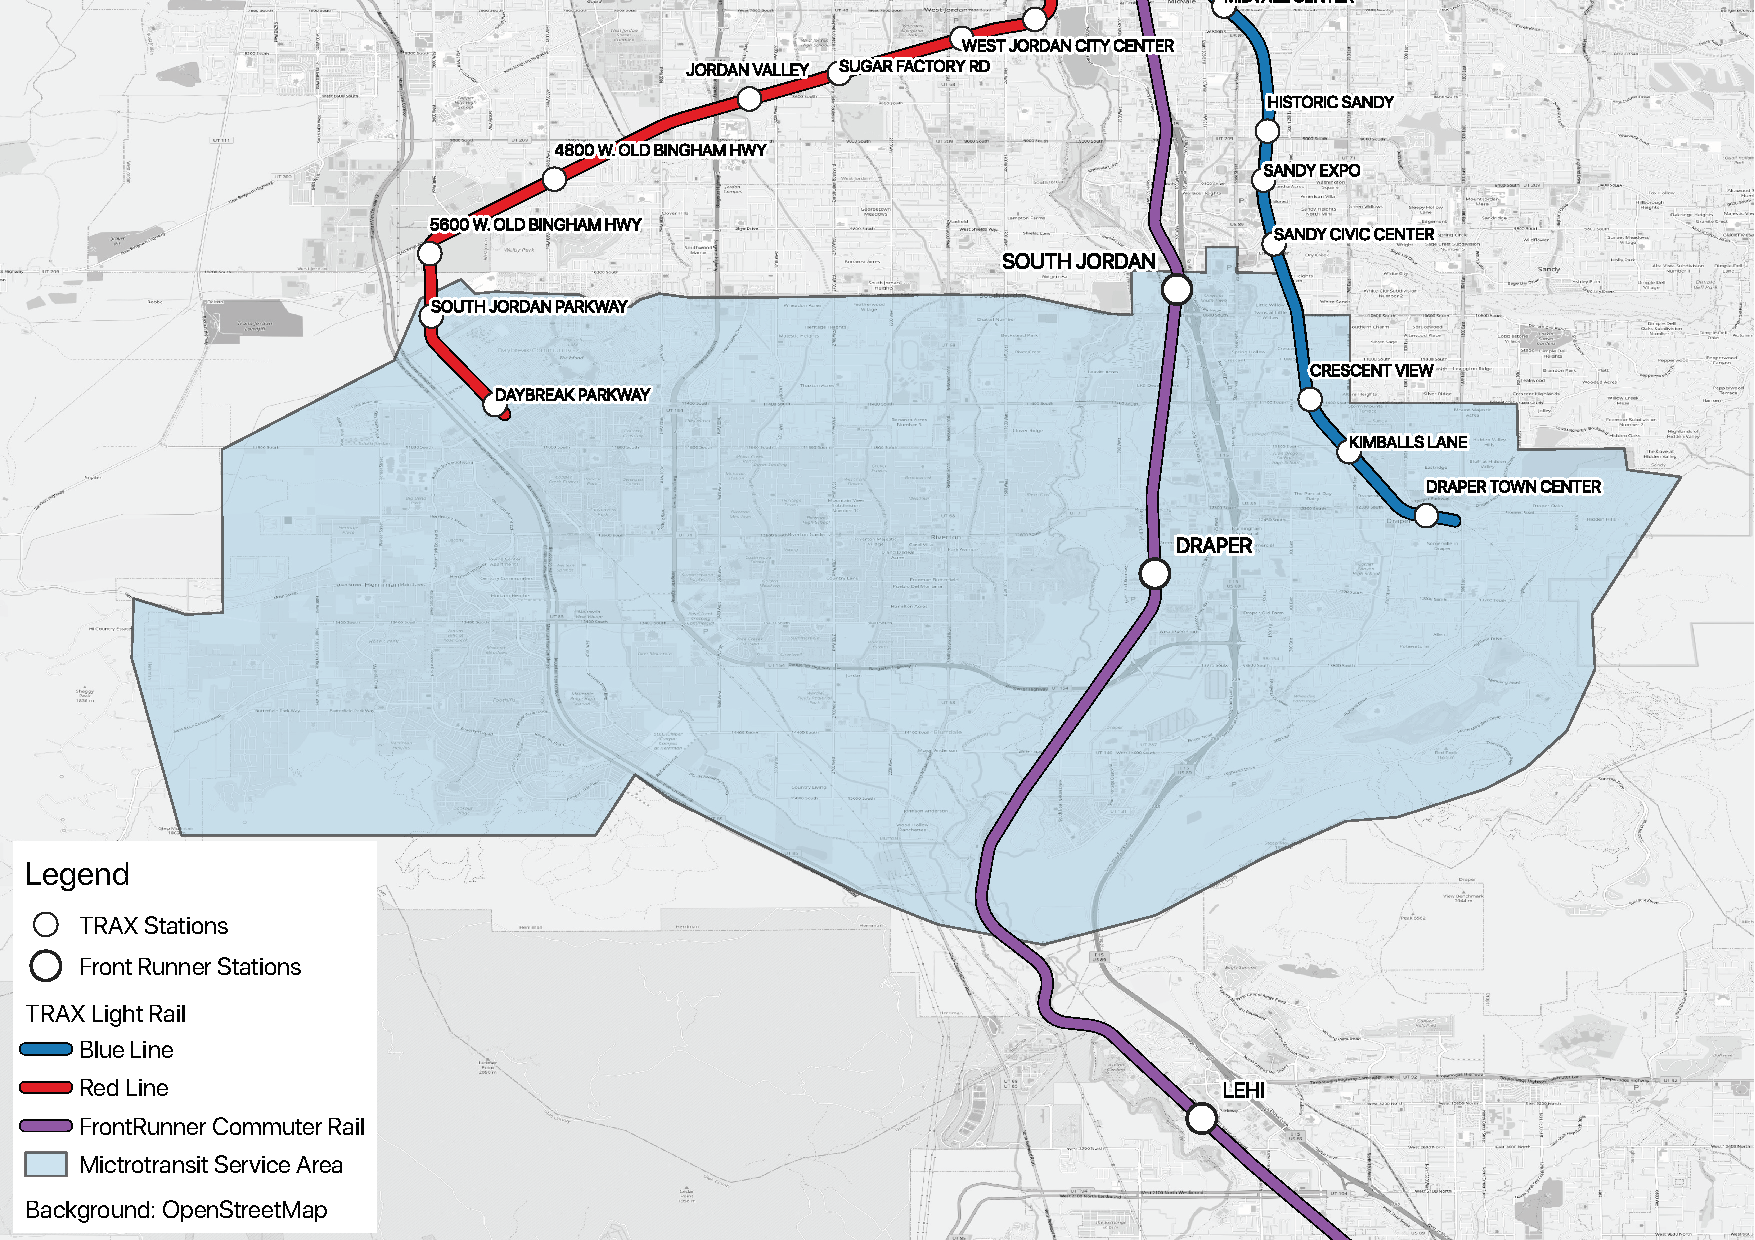
\includegraphics[width=1\linewidth]{images/service_area} \caption{UTA on-demand microtransit service area. Image by the authors}\label{fig:via-map}
\end{figure}

In establishing the on-demand microtransit service UTA partnered with Via, a
commercial mobility provider with new and ongoing operations in several US
cities. Passengers request rides using the VIA mobile application or calling a
designated service line and await the vehicle at a pickup point near to their
origin. Passengers share rides based on the availability of vehicles and the
compatibility of paths, as determined by algorithms embedded in the VIA service.
The vehicle will drop the passenger off near their destination or at TRAX or
FrontRunner stations; both the pickup and drop-off points must lie within the
service area shown in Figure \ref{fig:via-map}. The regular adult one-way fare
is \$2.50 and includes a limited transfer to the UTA fixed route transit system.
By the end of February 2020, the microtransit system was carrying about 316
passenger trips per weekday with an average wait time of 11 minutes per trip
\citet{uta2020}.

\hypertarget{survey-design}{%
\subsection{Survey Design}\label{survey-design}}

UTA's primary goal in executing this survey was to understand the effectiveness
of its marketing campaign to raise awareness and information of the new service.
This survey also provided an opportunity to inform additional riders and to
evaluate rider perceptions and characteristics both before and immediately after
the service launch. As such the survey was administered in two tranches. The
first tranche was conducted on November 6th, 13th, and 14th of 2019 through
on-platform intercept interviews at the Draper and South Jordan FrontRunner
stations as well as the Draper Town Center TRAX station. The second tranche was
collected on several weekdays between January 10th and March 4th, 2020, and was
collected through on-platform intercept interviews at the same stations in
addition to the Daybreak Parkway TRAX station and at designated microtransit
pick-up points near the aforementioned rail stations; a limited number of
interviews were also conducted on board the microtransit vehicles. Interviews
were conducted throughout the day, but with a focus on the PM peak commute
period. The number of interviews conducted during each time period for each
tranche is shown in Table \ref{tab:survey-times}.

\begin{table}[ht]
    \centering
    \caption{Surveys Collected by Time of Day}
    \label{tab:survey-times}
    \begin{tabular}{lcc}
    \toprule
    Day Period           & Before   Launch & After   Launch \\
    \midrule
    AM (6-10)            & 7               & 6              \\
    Mid-Day (10-4)       & 13              & 26             \\
    PM (4-7)             & 33              & 43             \\
    Evening (7-Midnight) & 2               & 0              \\
    TOTAL                & 55              & 75            \\
    \bottomrule
    \end{tabular}
\end{table}

The surveys were administered via electronic tablet using a questionnaire
developed in a web-based survey software. The survey questions were developed
with the help of UTA staff and an external consulting team. The relevant
variables and source questions for this study are shown in Table
\ref{tab:survey-summary}, in the order in which the questions were asked. After
asking the respondent about their awareness of the system, the interviewer would
give a brief explanation of the service before asking about the respondent's
likeliness to use the system. The questionnaire for the second tranche included
additional questions that were identified as being important after the first
tranche was collected; for example, the questions about income and household
size were added between the tranches. Further, questions in the second tranche
for respondents on train platforms and either at or on board the microtransit
service had slightly different wording to reflect the separate contexts. There
was also a set of questions requesting general feedback on the UTA service that
is not included in this study.

\begin{table}[ht]
\renewcommand{\arraystretch}{1.5}
    \centering
    \caption{Survey Questionnaire Summary}
    \label{tab:survey-summary}
\begin{tabular}{l p{0.4\textwidth}p{0.3\textwidth}}
\toprule
Variable          & Question Text                                                                                    & Response Type                                     \\
\midrule
Frequency         & How often do you ride UTA?                                                                       & Multiple choice with days   per week              \\
Purpose           & Where are you headed today?                                                                      & Multiple choice with   purposes plus text "other" \\
Access Mode       & How did you travel to your   UTA stop/station today?                                             & Multiple choice with modes   plus text "other"    \\
Awareness         & Had you heard about UTA On   Demand before today?                                                & Yes / No                                          \\
Likeliness        & How likely are you to   download the VIA app and use UTA On Demand?                              & Likert scale with five   "likely" levels          \\
Why Likely        & Why did you choose that   ranking?                                                               & Text response                                     \\
Use Purpose       & What types of trips do you   think you could use it for?                                         & Multiple choice with   purposes plus text "other" \\
Auto Availability & How many vehicles (cars,   trucks or motorcycles) are available in your household?               & Multiple choice with 0   through 4+               \\
Household Size    & Including you, how many   people live in your household?                                         & Numeric                                           \\
Race              & What is your race /   ethnicity?                                                                 & Mutiple choice allowing   multiple selection      \\
Income            & Which of the following BEST   describes your TOTAL ANNUAL HOUSEHOLD INCOME in 2019 before taxes? & Multiple choice in ranges                         \\
Smartphone        & Do you have a smartphone?                                                                        & Yes / No                                          \\
Age               & What is your age?                                                                                & Multiple choice in ranges    \\                    
\bottomrule
\end{tabular}
\end{table}

\hypertarget{applications}{%
\section{Applications}\label{applications}}

Some \emph{significant} applications are demonstrated in this chapter.

\hypertarget{example-one}{%
\subsection{Example one}\label{example-one}}

\hypertarget{example-two}{%
\subsection{Example two}\label{example-two}}

\hypertarget{final-words}{%
\section{Final Words}\label{final-words}}

We have finished a nice book.

% %%%%%%%%%%%%%%%%%%%%%%%%%%%%%%%%%%%%%%%%%%
% %% optional
% \supplementary{The following are available online at www.mdpi.com/link, Figure S1: title, Table S1: title, Video S1: title.}
%
% % Only for the journal Methods and Protocols:
% % If you wish to submit a video article, please do so with any other supplementary material.
% % \supplementary{The following are available at www.mdpi.com/link: Figure S1: title, Table S1: title, Video S1: title. A supporting video article is available at doi: link.}

\vspace{6pt}

%%%%%%%%%%%%%%%%%%%%%%%%%%%%%%%%%%%%%%%%%%
\acknowledgments{This project was sponsored by UTA through the BYU Civil Engineering Capstone
Program. The authors would like to thank Jaron Robertson and Shaina Quinn of
UTA and Sahar Shirazi and Kenny Ferrel of WSP for oversight and input
throughout the project.}

%%%%%%%%%%%%%%%%%%%%%%%%%%%%%%%%%%%%%%%%%%

%%%%%%%%%%%%%%%%%%%%%%%%%%%%%%%%%%%%%%%%%%
\conflictsofinterest{The authors declare no conflict of interest.}

%%%%%%%%%%%%%%%%%%%%%%%%%%%%%%%%%%%%%%%%%%
%% optional
\abbreviations{The following abbreviations are used in this manuscript:\\

\noindent
\begin{tabular}{@{}ll}
TNC & Transportation Network Company, e.g.~Uber, Lyft \\
UTA & Utah Transit Authority \\
\end{tabular}}


%%%%%%%%%%%%%%%%%%%%%%%%%%%%%%%%%%%%%%%%%%
% Citations and References in Supplementary files are permitted provided that they also appear in the reference list here.

%=====================================
% References, variant A: internal bibliography
%=====================================
%\reftitle{References}
%\begin{thebibliography}{999}
% Reference 1
%\bibitem[Author1(year)]{ref-journal}
%Author1, T. The title of the cited article. {\em Journal Abbreviation} {\bf 2008}, {\em 10}, 142--149.
% Reference 2
%\bibitem[Author2(year)]{ref-book}
%Author2, L. The title of the cited contribution. In {\em The Book Title}; Editor1, F., Editor2, A., Eds.; Publishing House: City, Country, 2007; pp. 32--58.
%\end{thebibliography}

% The following MDPI journals use author-date citation: Arts, Econometrics, Economies, Genealogy, Humanities, IJFS, JRFM, Laws, Religions, Risks, Social Sciences. For those journals, please follow the formatting guidelines on http://www.mdpi.com/authors/references
% To cite two works by the same author: \citeauthor{ref-journal-1a} (\citeyear{ref-journal-1a}, \citeyear{ref-journal-1b}). This produces: Whittaker (1967, 1975)
% To cite two works by the same author with specific pages: \citeauthor{ref-journal-3a} (\citeyear{ref-journal-3a}, p. 328; \citeyear{ref-journal-3b}, p.475). This produces: Wong (1999, p. 328; 2000, p. 475)

%=====================================
% References, variant B: external bibliography
%=====================================
\reftitle{References}
\externalbibliography{yes}
\bibliography{book.bib}

%%%%%%%%%%%%%%%%%%%%%%%%%%%%%%%%%%%%%%%%%%
%% optional

%% for journal Sci
%\reviewreports{\\
%Reviewer 1 comments and authors’ response\\
%Reviewer 2 comments and authors’ response\\
%Reviewer 3 comments and authors’ response
%}

%%%%%%%%%%%%%%%%%%%%%%%%%%%%%%%%%%%%%%%%%%
\end{document}

